\chapter{Theoretical background}
\section{Artificial neural networks}
An artificial neural network is a computing system inspired by the neural structure of the biological brain and its way of processing information. Such structure is able to ``learn'' how to solve certain problems or recognize patterns without being pre-programmed with rules how to do it. Artificial neural networks are main tool used in  deep learning, which is part of bigger family of machine learning \cite{deep_learning_bib}.

\begin{figure}[H]
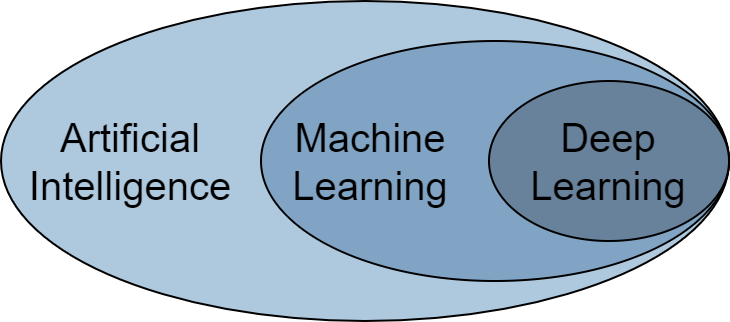
\includegraphics[width=8cm] {deep_learning_chart.png}
\centering
\caption{Deep learning belongingness}
\label{fig:deep_learning_chart}
\end{figure}

Fundamental unit of artificial neural network is so-called ``artificial neuron'' which is a mathematical function modeled after the structure of biological neuron \cite{artificial_neuron_bib}. Such artificial neuron has a number of inputs \(\{x_0, x_1, x_2, ..., x_n\}\) with assigned, separated weights \(\{w_0, w_1, w_2, ..., w_n\}\) for each of them to be multiplied by. In the simplest case, all product are summed and passed to a transfer function \(\varphi\). Additionally a bias value \(b\) is added to the sum of products which allows to shift the activation function up or down. Then the output \(y\) of the neuron is calculated as follows:
%
\begin{equation}
\label{eq:neuron_output}
y = \varphi\left(\sum_{j=0}^{n}x_jw_j\right)
\end{equation}
%
General idea of artificial neuron model is illustrated in figure \ref{fig:artificial_neuron_model}. Typically, neurons are organized into layers which may perform different operations. The output of neurons from one layer is passed to the input of the next layer or might be a part of output vector of whole network. Modern models of artificial neural networks may consist of tens or even hundreds of different layers, on which depends how well given network will cope with certain tasks. Those layers, during process of network training, can adjust theirs weights to produce output values that correctly solve given problem \cite{artificial_neuron_bib} \cite{artificial_neural_networks_bib}.

\begin{figure}[H]
\includegraphics[width=12cm] {artificial_neuron_model.png}
\centering
\caption{Artificial neuron model}
\label{fig:artificial_neuron_model}
\end{figure}

Artificial neural networks have found many, different applications in various fields, in both, academic and business environments. For some time, they are successfully used to solve problems of system identification and control (processes in industrial sector), image classification (medical diagnosis), financial forecasting, face recognition (security), sequence recognition (speech recognition), pattern recognition (data generation) and many more \cite{ann_applications_bib}.

\section{Convolutional neural networks}
One of the most commonly applied type of deep neural networks, in case of image processing problems, are the convolutional neural networks. CNNs are constructed with convolutional layers that consist of a certain amount of filters, which allow them to effectively ``recognize'' patterns such as edges, curves, shapes, textures and colors \cite{convolutional_networks_bib}. One of the most important property of such networks is ability to learn spatial hierarchies of patterns. First layer learns to recognize simple features like edges or curves. Filters of following layers can learn more complex patterns made of features from previous layers, like for example circles, squares, eyes, faces and so on \cite{deep_learning_with_python_bib}. Another significant property of CNNs is the fact that the patterns they learn are translation invariant, which means that pattern learned in one part of the picture can be recognized anywhere else.\\

Due to its pattern-recognition abilities, convolutional neural networks have found many, different applications in various fields \cite{cnn_applications_bib}. Depending on the input data dimensionality, CNNs might be applied to time series prediction (weather forecast) or signal identification (ECG signal identification) in case of f one-dimensional data. Two-dimensional CNNs are very effective with image classification (breast cancer tissues classification), object detection (autonomous vehicles) and face recognition (security). In theory, CNNs might be applied to data with any number of dimensions but it is not a popular approach as such data is hard to understand for humans.\\

The main idea behind the convolutional layer is a mathematical operation called convolution, which is a combination of two functions that produces third function. In case of CNNs, convolution is performed by sliding given filter (in form of matrix), also known as kernel, over input data. At every point of input data, a matrix multiplication is calculated and sums the result onto the feature map \cite{convolution_operation_bib}. This process is illustrated in figure \ref{fig:convolution}, where exemplary filter, applied on input data produces convolved feature (also called feature map).

\begin{figure}[H]
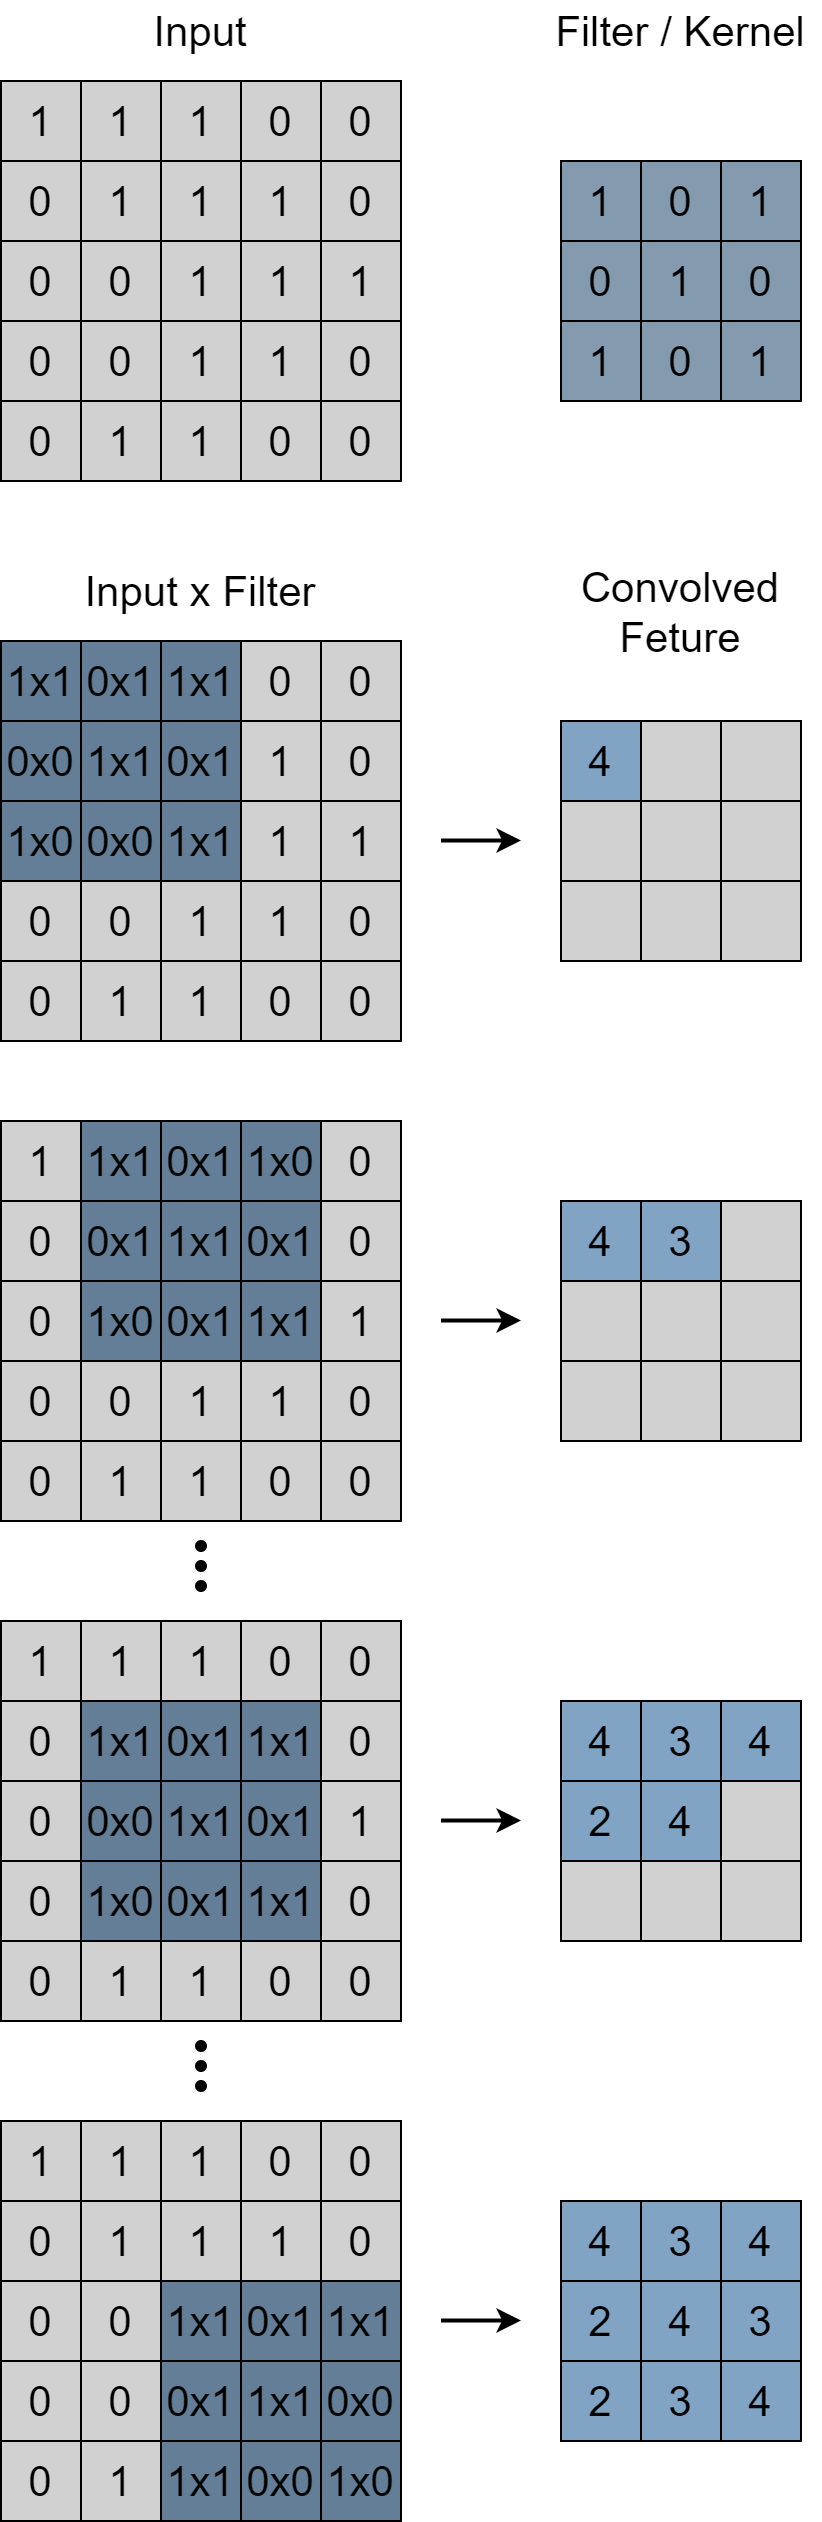
\includegraphics[height=\textheight] {convolution.png}
\centering
\caption{Convolution operation}
\label{fig:convolution}
\end{figure}

\section{Types of machine learning algorithms}
Depending on the problem specification and the form of related training data, different algorithms might be used for the process of artificial neural networks training. The most common types of training methods are: supervised, unsupervised, semi-supervised and reinforcement learning \cite{algorithms_types_bib} \cite{algorithms_types2_bib}.\\

The most popular paradigm for machine learning, supervised learning, is applied in case of well-labeled data and is typically used for classification problems. This approach aims to find a function that maps an input to an output based on example input-output pairs. Thanks to the loss function, that measures the accuracy of the network by comparing its outcome with responding labels, model updates its weights to produce more accurate predictions. A significant disadvantage of this approach is the need for large amount of well-labeled data, necessary for training efficient networks. Another very popular type of training, perfect in case of unlabeled data, is unsupervised learning also known as self-organization. The goal of this approach is to model the underlying structure or distribution in the data without human supervision (in form of labeled data). This learning type is best suited for clustering problems where certain relationships in data occur.\\

A method that combines supervised and unsupervised learning is called semi-supervised learning. The idea is to pre-train models on small amount of labeled data and later use large amount of unlabeled data to increase accuracy and improve generalization skills of trained networks. Such approach allows to harness information from gathered data without spending a lot of time on labeling all of them.

\section{Haar feature-based cascade classifier}
\label{Haar feature-based cascade classifier}
To be able to extract faces from videos, Haar feature-based cascade classifier was used. This detector, provided by OpenCV library \cite{opencv_haar_bib}, is based on Paul Viola's and Michael Jones's method \cite{Haar_bib} which involves detecting and marking in the image certain characteristic features of human face, in the form of black and white, adherent rectangles, as illustrated in the figure \ref{fig:haar_example}. Afterwards, thanks to the Viola-Jones method, out of many weak classifiers (features), a chain of filters is created (cascade), in which single filter is responsible for detecting single feature. If the given part of an image called window positively passes through all the filters of the cascade, than this window is considered to contain face.

\begin{figure}[H]
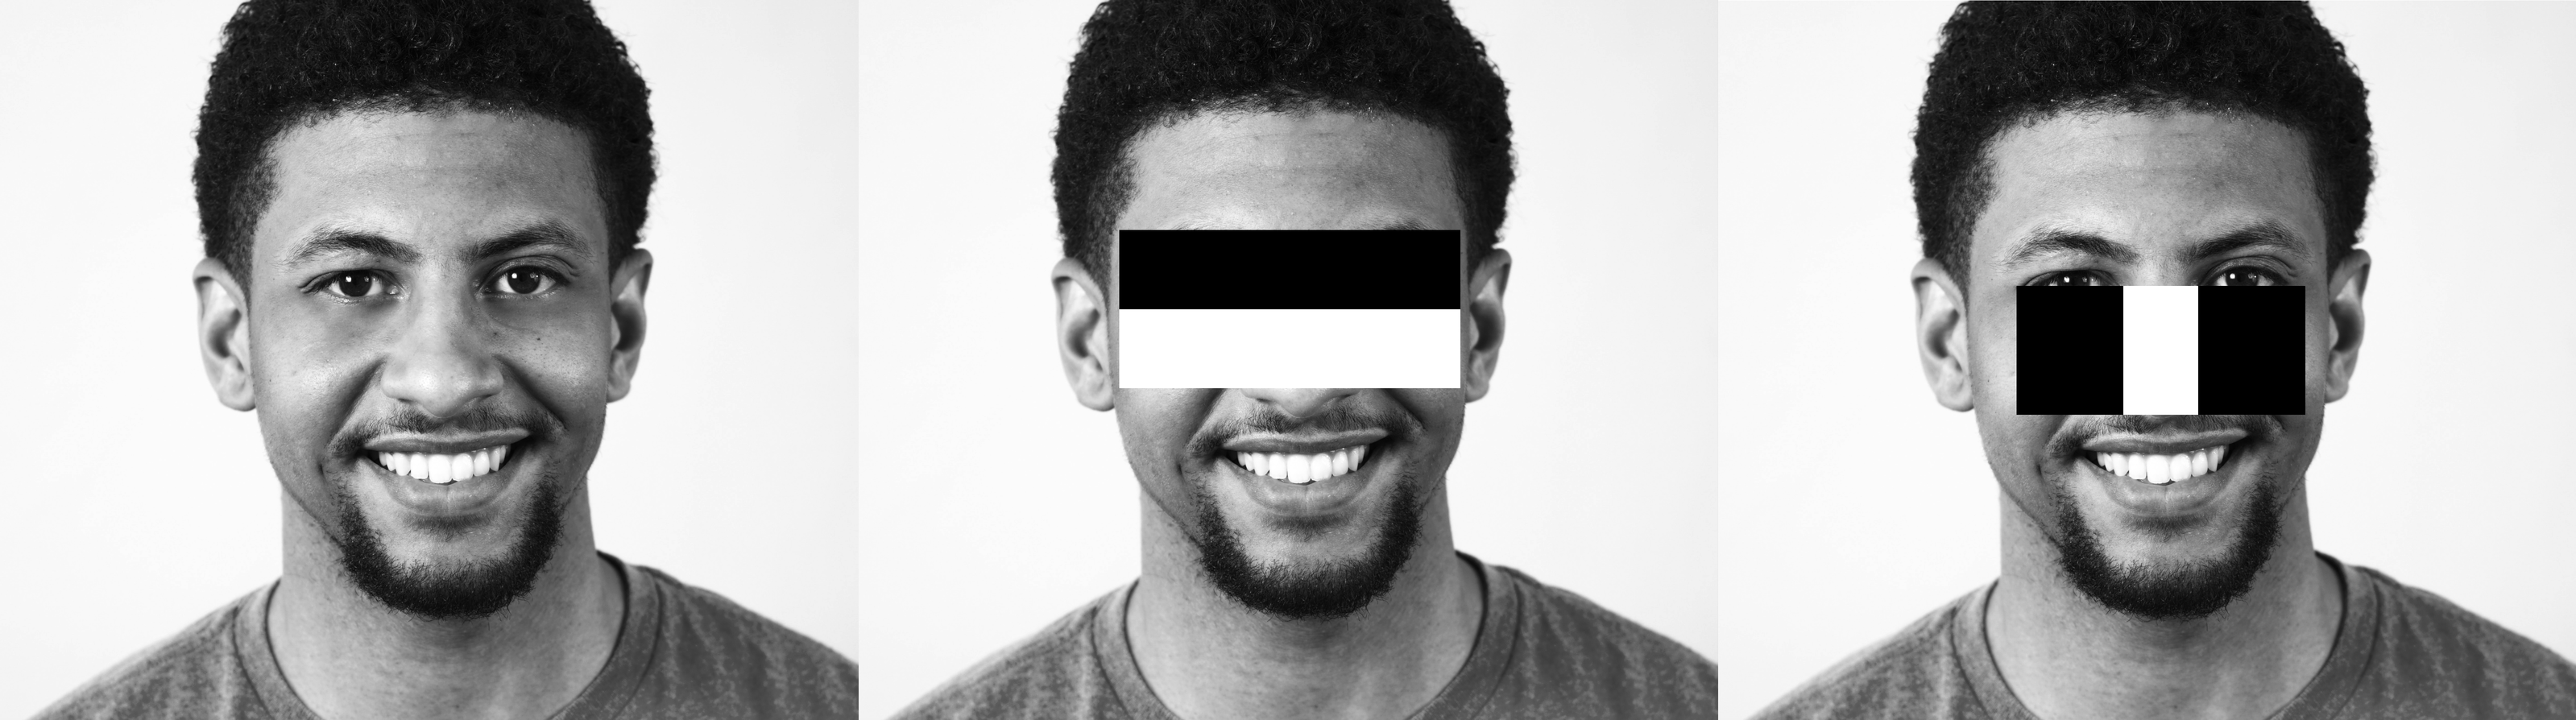
\includegraphics[width=\textwidth] {haar_example.png}
\centering
\caption{Example of Haar-like features detection}
\label{fig:haar_example}
\end{figure}